\documentclass{article}
\usepackage[a4paper,margin=1in,footskip=0.25in]{geometry}
\usepackage{tikz}
\usetikzlibrary{spy,shapes,shadows,calc,pgfplots.groupplots}
\usepackage{amsmath}
\usepackage{amsfonts}
\usepackage{amssymb}
\usepackage{stmaryrd}
\usepackage{graphicx}
\usepackage{epstopdf}
\usepackage{algorithmic}
\usepackage{enumitem}
\usepackage{booktabs}
\usepackage{pgfplotstable}
\usepackage{colortbl}

\pgfplotstableset{% global config
    every head row/.style={before row=\bottomrule,after row=\hline},
    every last row/.style={after row=\toprule},
}

\providecommand{\abs}[1]{\left\lvert#1\right\rvert}
\providecommand{\norm}[1]{\left\lVert#1\right\rVert}

\newcommand{\drawSquare}{\begin{tikzpicture}
\node[ ] at (0,0) {\textcolor{blue}{\nullfont\pgfuseplotmark{square}}};
\end{tikzpicture} }
\newcommand{\drawCircle}{
\begin{tikzpicture}
\node[ ] at (0,0) {\textcolor{red}{\nullfont\pgfuseplotmark{o}}};
\end{tikzpicture} }
\newcommand{\drawTriangle}{\begin{tikzpicture}
\node[ ] at (0,0) {\textcolor{green!70!black}{\nullfont\pgfuseplotmark{triangle}}};
\end{tikzpicture}
}
\begin{document}

\begin{figure}[h]
\centering
\begin{tikzpicture}[scale = 1.0]
\begin{scope}[ ]
\begin{tiny}
\begin{axis}[
    height = 4.75cm,
    width = 5.7cm,
    name=displ,
    ymode=log,
    xmode=log,
    ymax = 2e-1,
    axis y line*=left,
    xlabel= { $\Delta t = h$},
    x label style={at={(axis description cs:0.35,+0.225)},anchor=east},
    legend style = { column sep = 10pt, legend columns = 1, legend to name = grouplegend,},
    title style={at={(0.5,1.0735)},anchor=north},
    title = {  $\norm{ u - \mathcal{L}_{\Delta t} \underline{u}_1 }_{L^{\infty}(0,T;L^2(\Omega))}$ },
    legend style={at={(0.5,-0.1)},anchor=north},
	]
    
    \addplot[blue,only marks,mark=square,mark options={scale=1.25},forget plot] 
   	table[x=deltat,y=MTM-lo] {../data/precond-3d-GCC-LinftyL2u-order1.dat}; %\addlegendentry{$q=1$}%   
    \addplot[blue,very thick] 
   	table[x=deltat,y=MTM-lo] {../data/precond-3d-GCC-LinftyL2u-order1.dat}; \addlegendentry{$q=1$}%   
     \addplot[red,very thick,only marks, mark=o,mark options={scale=1.25},forget plot] 
   	table[x=deltat,y=DFB] {../data/precond-3d-GCC-LinftyL2u-order1.dat}; 
    
    \addplot[blue,only marks,mark=square,mark options={scale=1.25},forget plot] 
   	table[x=deltat,y=MTM-lo] {../data/precond-3d-GCC-LinftyL2u-order2.dat}; %\addlegendentry{$q=2$}%    
    \addplot[blue,very thick,dashed] 
   	table[x=deltat,y=MTM-lo] {../data/precond-3d-GCC-LinftyL2u-order2.dat}; \addlegendentry{$q=2$}%   
     \addplot[red,very thick,only marks, mark=o,mark options={scale=1.25},forget plot] 
   	table[x=deltat,y=DFB] {../data/precond-3d-GCC-LinftyL2u-order2.dat}; 

    \addplot[blue,only marks,mark=square,mark options={scale=1.25},forget plot] 
   	table[x=deltat,y=MTM-lo] {../data/precond-3d-GCC-LinftyL2u-order3.dat}; %\addlegendentry{$q=3$}%   
    \addplot[blue,very thick,densely dotted] 
   	table[x=deltat,y=MTM-lo] {../data/precond-3d-GCC-LinftyL2u-order3.dat}; \addlegendentry{$q=3$}%   
    \addplot[red,very thick,only marks, mark=o,mark options={scale=1.25},forget plot] 
   	table[x=deltat,y=DFB] {../data/precond-3d-GCC-LinftyL2u-order3.dat}; 

    \addplot[lightgray,dashed,ultra thick] 
    	table[mark=none,x=deltat,y expr ={.15*\thisrowno{0}}] {../data/precond-3d-GCC-LinftyL2u-order1.dat};  %\addlegendentry{$ \mathcal{O}(\Delta t) $ } %
    \addplot[lightgray,dotted,ultra thick] 
    	table[mark=none,x=deltat,y expr ={.15*\thisrowno{0}*\thisrowno{0} }] {../data/precond-3d-GCC-LinftyL2u-order2.dat};  %\addlegendentry{$ \mathcal{O}((\Delta t)^2) $ } %
    \addplot[lightgray,dashdotted,ultra thick] 
    	table[mark=none,x=deltat,y expr ={.05*\thisrowno{0}*\thisrowno{0}*\thisrowno{0}}] {../data/precond-3d-GCC-LinftyL2u-order3.dat};  %\addlegendentry{$ \mathcal{O}((\Delta t)^3) $ } %
    %\legend{ $q=k=1$, $q=k=2$,$q=k=3$ } 
    %\node[draw,circle,ultra thick,lightgray] (Z1) at (axis cs:0.0625,4.5e-3) {};
   \end{axis}
    \node at ($(displ) + (-0.0cm,-2.55cm)$) {\ref{grouplegend}}; 
\end{tiny}
\end{scope}

 \begin{scope}[xshift=4.5cm]
 %\begin{footnotesize}
 \node (geom) at (1.0,2.25) {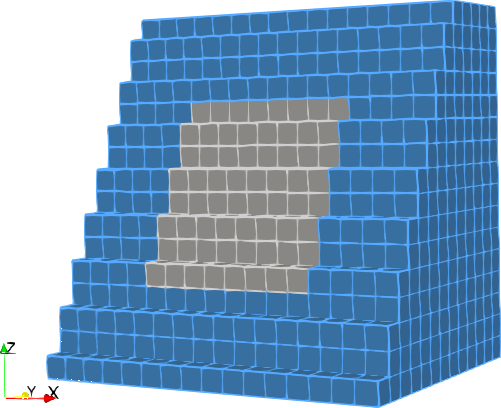
\includegraphics[scale =.15]{GCC-data-domain-reflvl3.png}};
 \node[draw,fill=white] (la) at (1.15,3.25) { {\footnotesize $\omega $ }};
  \node[] (Z2) at (-2.25,0.55) {};
  \node (err) at (1.25,-0.4) {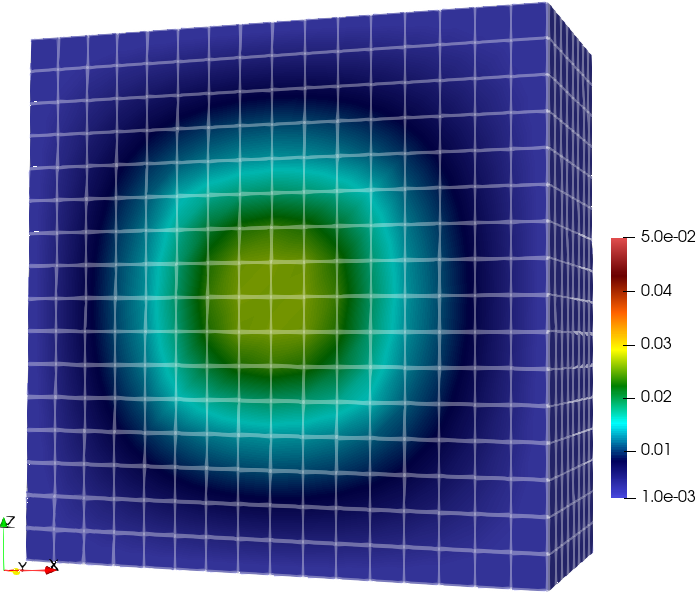
\includegraphics[scale =.115]{GCC-abserr-displacement-reflvl3.png}};
 \node[draw,fill=white] (la) at (1.05,0.875) {\tiny{$\vert u(0,\cdot) - \mathcal{L}_{\Delta t} \underline{u}_1(0,\cdot) \vert$}};
  \draw[lightgray,ultra thick, ->] (-0.3,-0.55 ) -- (-3.145, 1.695);
 %\end{footnotesize}
 \end{scope}

\begin{scope}[xshift=7.5cm]
\begin{tiny}
\begin{axis}[ 
    height = 4.75cm,
    width = 5.7cm,
    name=vel,
    ymode=log,
    xmode=log,
    ymax = 1e-0,
    axis y line*=left,
    xlabel= { $\Delta t = h$},
    legend style = { column sep = 10pt, legend columns = 1, legend to name = grouplegendv,},
    x label style={at={(axis description cs:0.35,+0.225)},anchor=east},
    title style={at={(0.5,1.0735)},anchor=north},
    title = {  $\norm{ \partial_t( u - \mathcal{L}_{\Delta t} \underline{u}_1 ) }_{L^{2}(0,T;L^2(\Omega))}$ },
    legend style={at={(0.5,-0.1)},anchor=north},
	]
    
    \addplot[blue,only marks,mark=square,mark options={scale=1.25},forget plot] 
   	table[x=deltat,y=MTM-lo] {../data/precond-3d-GCC-L2L2ut-order1.dat}; %\addlegendentry{$q=1$}%   
    \addplot[blue,very thick,forget plot] 
   	table[x=deltat,y=MTM-lo] {../data/precond-3d-GCC-L2L2ut-order1.dat}; %\addlegendentry{$q=1$}%   
     \addplot[red,very thick,only marks, mark=o,mark options={scale=1.25},forget plot] 
   	table[x=deltat,y=DFB] {../data/precond-3d-GCC-L2L2ut-order1.dat}; 
    
    \addplot[blue,only marks,mark=square,mark options={scale=1.25},forget plot] 
   	table[x=deltat,y=MTM-lo] {../data/precond-3d-GCC-L2L2ut-order2.dat}; %\addlegendentry{$q=2$}%    
    \addplot[blue,very thick,dashed,forget plot] 
   	table[x=deltat,y=MTM-lo] {../data/precond-3d-GCC-L2L2ut-order2.dat}; %\addlegendentry{$q=2$}%   
     \addplot[red,very thick,only marks, mark=o,mark options={scale=1.25},forget plot] 
   	table[x=deltat,y=DFB] {../data/precond-3d-GCC-L2L2ut-order2.dat}; 

    \addplot[blue,only marks,mark=square,mark options={scale=1.25},forget plot] 
   	table[x=deltat,y=MTM-lo] {../data/precond-3d-GCC-L2L2ut-order3.dat}; %\addlegendentry{$q=3$}%   
    \addplot[blue,very thick,densely dotted,forget plot] 
   	table[x=deltat,y=MTM-lo] {../data/precond-3d-GCC-L2L2ut-order3.dat}; %\addlegendentry{$q=3$}%   
    \addplot[red,very thick,only marks, mark=o,mark options={scale=1.25},forget plot] 
   	table[x=deltat,y=DFB] {../data/precond-3d-GCC-L2L2ut-order3.dat}; 
 
    \addplot[lightgray,dashed,ultra thick] 
    	table[mark=none,x=deltat,y expr ={1.3*\thisrowno{0}}] {../data/precond-3d-GCC-L2L2ut-order1.dat};  \addlegendentry{$ \mathcal{O}(\Delta t) $ } %
    \addplot[lightgray,dotted,ultra thick] 
    	table[mark=none,x=deltat,y expr ={1.4*\thisrowno{0}*\thisrowno{0} }] {../data/precond-3d-GCC-L2L2ut-order2.dat};  \addlegendentry{$ \mathcal{O}((\Delta t)^2) $ } %
    \addplot[lightgray,dashdotted,ultra thick] 
    	table[mark=none,x=deltat,y expr ={.5*\thisrowno{0}*\thisrowno{0}*\thisrowno{0}}] {../data/precond-3d-GCC-L2L2ut-order3.dat};  \addlegendentry{$ \mathcal{O}((\Delta t)^3) $ } %
    %\legend{ $q=k=1$, $q=k=2$,$q=k=3$ } 
    %\node[draw,circle,ultra thick,lightgray] (Z1) at (axis cs:0.0625,6.5e-3) {};
   \end{axis}
    \node at ($(vel) + (-0.0cm,-2.55cm)$) {\ref{grouplegendv}}; 
\end{tiny}
\end{scope}
\end{tikzpicture}
\label{fig:GCC-3D}
\end{figure}

\end{document}

